\section{Produktdaten}

\textbf{/D201/} Zum Speichern der MNIST-Bilder werden die folgenden Daten persistiert:

\begin{tabular}{cl}
(1) & id: UUID \\[0.2cm]
(2) & Name des Bildes: string\\[0.2cm]
(3) & Typ des Bildes (Training, Test): string\\[0.2cm]
(4) & die abgebildete Ziffer: int\\[0.2cm]
(5) & die Bildnummer: int\\[0.2cm]
(6) & base64-codiertes Bild: string.\\[0.2cm]  
\end{tabular}

\textbf{/D203/} Für jedes neuronale Netz werden die folgenden Daten gespeichert: 

\begin{tabular}{cl}
(1) & id: string \\[0.2cm]
(2) & Name des neuronalen Netzes: string\\[0.2cm]
(3) & Beschreibung des neuronalen Netzes: string\\[0.2cm]
(4) & Typ Neuronalen Netzwerkes (Prod, Test): string \\[0.2cm]
(5) & alle Ids der im Neuronalen Netz enthaltenen Layer: map<int, layer>\\[0.2cm]
(6) & alle im Netz vorhandenen Axone: map<string, axon>.\\[0.2cm]
\end{tabular}

Für jeden Layer eines neuronalen Netzes werden die folgenden Daten gespeichert: 

\begin{tabular}{cl}
(1) & id: string \\[0.2cm]
(2) & Dimension (in x- und y-Richtung) des Layers: int \\[0.2cm]
(3) & alle Ids der im Layer enthaltenen Knoten: map<int, node>.\\[0.2cm]
\end{tabular}

Für jeden Knoten eines Layers werden die folgenden Daten gespeichert: 

\begin{tabular}{cl}
(1) & id: string \\[0.2cm]
(2) & der Bias: double \\[0.2cm]
(4) & die Aktivierungsfunktion: string.\\[0.2cm]
\end{tabular}

Für jedes Kindaxon eines Knotens werden die folgenden Daten gespeichert: 

\begin{tabular}{cl}
(1) & das Gewicht eines Axons: double \\[0.2cm]
(2) & die Elternknotenid: string \\[0.2cm]
(3) & die Kindknotenid: string. \\[0.2cm]
\end{tabular}

Zur Persistenz der gesamten oben aufgeführten Daten eines neuronalen Netzes werden die in Abb. \ref{fig_dbClassdiagram} dargestellten Datenstrukturen verwendet und in einer MongoDB abgelegt. 
\begin{figure}[h]
\begin{center}
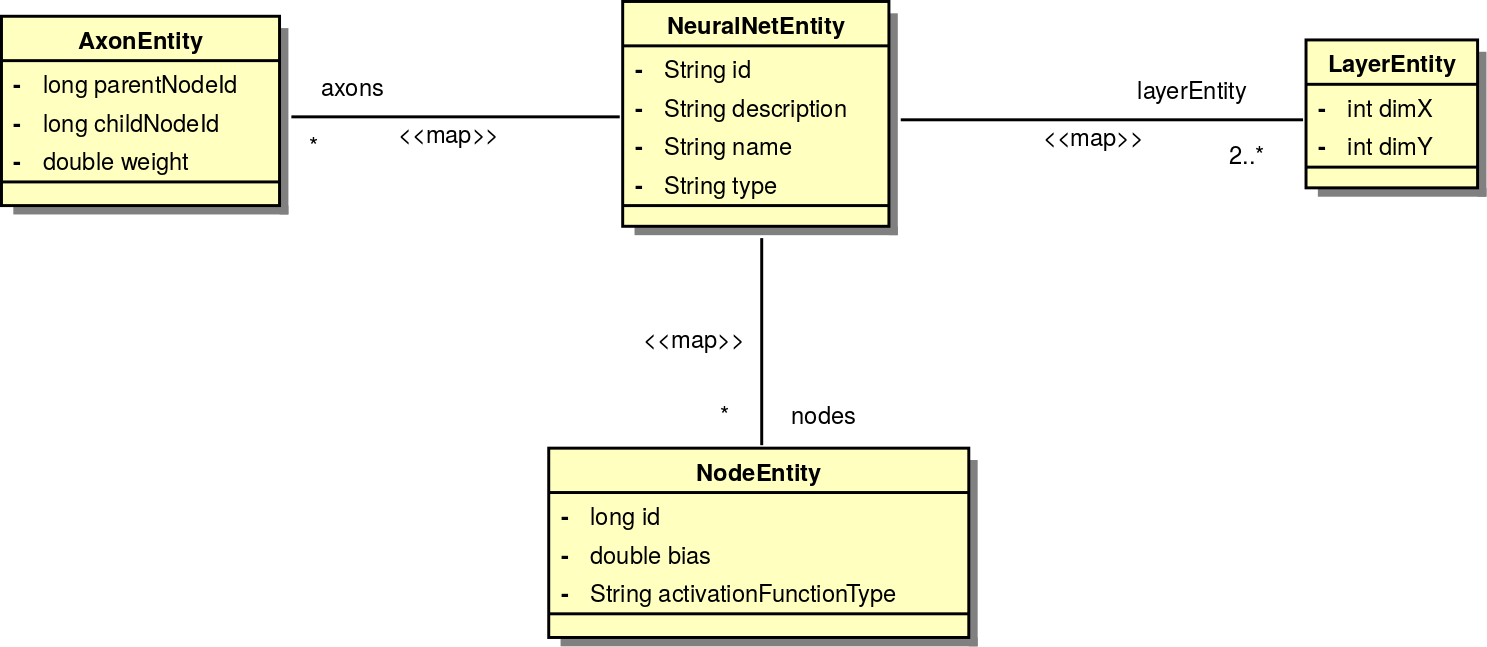
\includegraphics[width=\textwidth]{Abbildungen/UML/jan/datenBankKlassendiagramm.png}
\caption{Klassendiagramm der zur Persistierung eines neuronalen Netzes benötigten Datenstrukturen.}
\label{fig_dbClassdiagram}
\end{center}
\end{figure}
Es ist zu beachten, dass die Objekte dabei nicht als unabhängige, in Beziehung stehende Entitäten\footnote{Dies entspräche dem Vorgehen für eine relationale Datenbank. Durch die vielen zirkulären Referenzen ist dieser Zugang nicht geeignet.} in der Datenbank sondern als ein einziges Json-Objekt abgelegt werden. 
